\title{Collider: A mobile app for particle physics outreach}
\author{Tom McLaughlan}
\date{\today}

\documentclass[12pt]{article}
\usepackage{graphicx}

\begin{document}
\maketitle

\section{Introduction}
Collider is a cross platform event display for the ATLAS experiment, designed to run on the mobile platforms Android and iOS.
The main aim of Collider is to bring understanding of the physics at ATLAS to a wider audience through the use of online learning materials and games. Collider builds on the success of \emph{LHSee}, an existing app for Android devices, and extends the scope of 
the app by adding iOS support.

\section{Implementation}
Collider is developed in C++ using the Marmalade\cite{marmalade} and IwGame\cite{iwgame} platforms, which allows for compilation to 
binary for both Android and iOS, as well as other platforms dependant on licensing. Within this framework, OpenGL-ES 1.0 is utilised 
to provide the 3D drawing capability required for rendering the ATLAS detector and event data.

\subsection{Rendering the ATLAS detector}
The ATLAS Event Display, ATLANTIS\cite{atlantis}, provides a publicly available representation of the ATLAS geometry in XML format. This 
geometry provides the position and size of the various components of ATLAS, which Collider interprets in order to produce its own 
representation. The Inner Detector and Muon Spectrometer are the most complex components of the detector.

The Inner Detector comprises several concentric hollow cylinders in the barrel region and several discs in the endcaps. The Muon 
Spectrometer consists of a series of boxes arranged in concentric cylinders in the barrel, and two discs on each endcap.
By contrast, the Electromagnetic Calorimeter is a single cylinder.

\subsection{Rendering the ATLAS data}
Data from ATLAS are stored in a similar XML format, again provided by ATLANTIS. The data shown in Collider are Inner Detector and Muon tracks, binned calorimeter data and electrons.

The tracks are drawn by simply joining several vertices with a line. For Muon tracks, this is provided by the `polyline' data, while for 
Inner Detector tracks, a helix is generated from the track parameters.
Calorimeters are binned in $\phi$ and $\eta$, and are drawn as boxes, with the extension from the centre determined by the amount of energy in the calorimeter.
Electrons are drawn simply as cones, oriented in $\eta\phi$, intended to highlight the track and calorimeter activity an electron is expected to leave in the detector. 

\subsection{Defining a Game in Collider}
Games in Collider are a combination of the event display, showing a predetermined list of events, and a multiple choice answer bank. 
The user plays the game by analysing the event and deciding from the multiple choices which answer best describes the event. Once the 
user has chosen an answer for each event, the results can be collected.
\\
In order to create a game for Collider, there are three steps to follow (see appendix \ref{makegame} for full details):
\begin{itemize}
\item Compile a list of events and answers in the designated XML format
\item Create an icon for the game
\item Add the game to the LandingScreen.xml game list
\end{itemize}

\section{Impact}

Collider has, in the first weeks of release, already generated interest among users of Twitter and Facebook. The scope of this impact can been seen in download statistics for both platforms.

\subsection{Android statistics}
\begin{figure}
\centering
    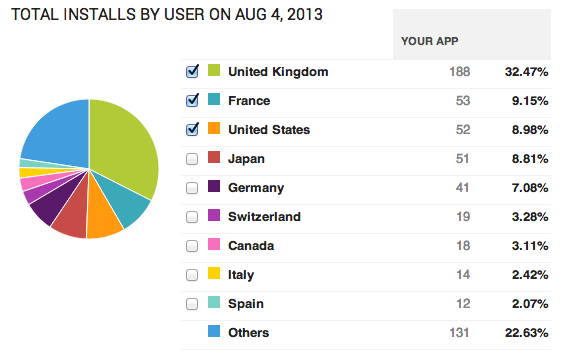
\includegraphics[width=0.8\textwidth]{img/androidcountries.png}
    \caption{\label{fig:androidcountries}Number of Android installs by country in which the device was registered.}
\end{figure}
The Android version of the app has amassed 579 downloads since July 23rd 2013. By country in which the device was registered, this breaks down as shown in figure \ref{fig:androidcountries}.
In addition, there have been four user reviews at the time of writing, all of which rate Collider at 5 stars (of a possible 5).

\subsection{iOS statistics}
\begin{figure}
\centering
    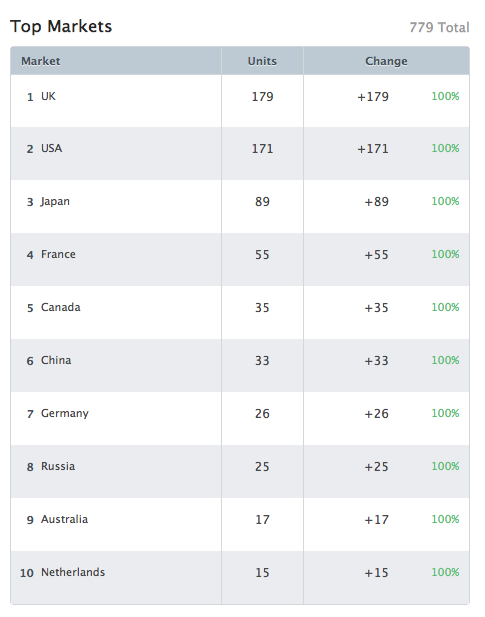
\includegraphics[width=0.8\textwidth]{img/ioscountries.png}
    \caption{\label{fig:ioscountries}Number of iOS installs by country in which the device was registered.}
\end{figure}
The iOS version of the app has been downloaded over 700 times since release on August 2nd 2013. The breakdown by country is shown 
in figure \ref{fig:ioscountries}.

\subsection{Website Analytics}
The website developed alongside the app is designed to be both a landing page for Collider from a desktop computer, allowing people to find out about Collider and how to download it, as well as being a help page to be accessed within Collider itself.

\begin{figure}
\centering
    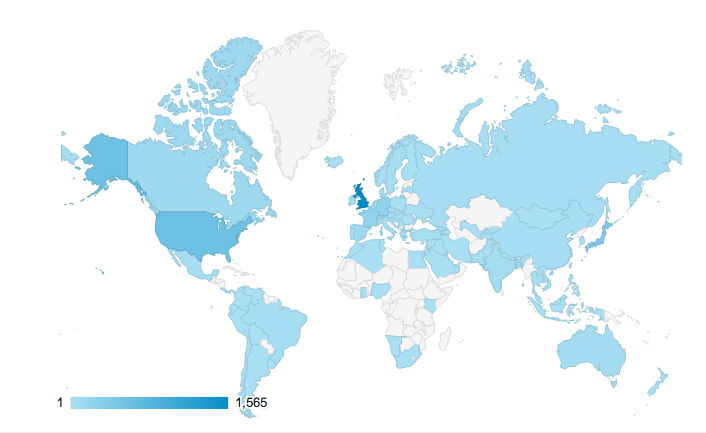
\includegraphics[width=0.8\textwidth]{img/webmap.png}
    \caption{\label{fig:webmap}Visitors to the website by user location.}
\end{figure}

Google Analytics allows us to track user interaction with the website, from both within the app and from desktop computers. This works by recording hits to the website with location and device information.
The number of hits to the website since launch, broken down by country, is shown in figure \ref{fig:webmap}. The majority of visitors are based in the UK, with the US and Japan in second and third place respectively.

\begin{figure}
\centering
    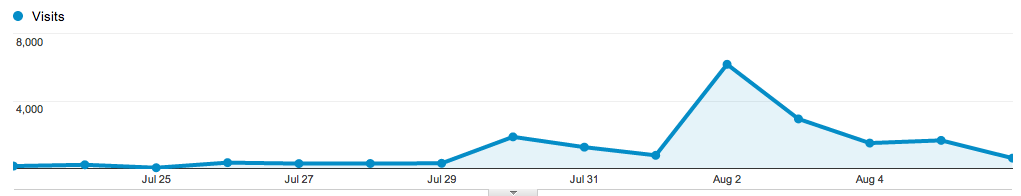
\includegraphics[width=0.8\textwidth]{img/apphits.png}
    \caption{\label{fig:apphits}Interactions within the app by day.}
\end{figure}

Within the app itself, there is some analytics tracking code. Each time the event display loads or closes, a `virtual webpage' is loaded, sending the tracking data to Google Analytics. This shows up just as a webpage view would, only for `virtual webpages'. This allows tracking of interaction with the app itself, interpreted as the number of times the event display is opened/closed\footnote{The event display is closed and reopened whenever a new event is loaded, so this interaction also counts as a hit.}
Figure \ref{fig:apphits} shows the number of interactions per day within the app. The peak at August 2nd coincides with the iOS release of Collider.

\appendix
\section{Extending Collider}
Collider was developed with a fixed timescale in mind. This led to the unavoidable fact that many proposed features could not be completed in time for the release of the app. Detailed in this appendix are some of the possible new features to add to Collider in the future.

\subsection{Adding new Games}
A Game in Collider is constructed with a simple XML format, and every game is constructed in the same way, meaning it is trivial for 
a new game to be added at anytime (see Appendix \ref{app:code} for more information on how to construct a game).
This method of creating new games is dependent on a developer inserting the game into the codebase, compiling the app again and completing the App Store submission processes again and again.

A simple way to get around this would be to add the capability to download new games from within Collider, letting the app itself do 
the work of downloading the XML file and inserting the game into the games list.

\subsection{Invariant Mass Calculation}
The data visualised by Collider contains enough information to do some basic calculations such as the invariant mass of a decaying 
particle (e.g.~A Z boson decaying to two electrons). This calculation already exists in the app, though a way of displaying the data is missing.
In testing, this feature sent the result of the calculation to a server, which ran a plotting script every 5 minutes. The resulting histogram was then stored on a webpage which was viewable within the app.
This method is fine for multiple users collaborating on a single measurement, but with the large amount of users expected for Collider, 
a single histogram from a fixed set of data is not feasible.

To get around this, an in app histogram tool could be implemented, which allows each user to have their own histogram compiled as the play the game.


\section{Code Overview}
\label{app:code}
\subsection{Setting up the environment}
Collider is written in C++, using Marmalade 6.3 and IwGame 0.370. As IwGame is open source, some modifications to the IwGame code have been made to ensure compatibility with Marmalade 6.3, including a change to the version of libpng used. Collider will NOT compile without the exact version of IwGame stored in the SVN repository at:
\begin{verbatim}
svn+ssh://USERNAME@svn.cern.ch/reps/lhsee
\end{verbatim}

To set up the environment open the GameSceneGL.mkb. This should open with a program called `MKB', which should have been installed with the Marmalade framework. On Mac OSX, this will open XCode. In Windows, this will open Microsoft Visual C++.

\subsection{Creating a Game}
Games in Collider are XML files consisting of a Game title, list of events and answers, and URL to be accessed in the in game browser.
The structure of a game is as follows:
\footnotesize
\begin{verbatim}
<xml>
    <ClassificationGame name="Tutorial" tutorial="true" 
       author="Tom McLaughlan" level="1">
        <Link title="Online Help" 
            url="http://collider.physics.ox.ac.uk/detecting.html"/>
        <Event type="Electron" file="electron.xml"/>
        <Event type="Muon" file="muon.xml"/>
        <Event type="Jet" file="jet.xml"/>
        <Event type="Neutrino" file="neutrino.xml"/>
    </ClassificationGame>
</xml>
\end{verbatim}
\normalsize
The \emph{level} parameter determines the `difficulty' of the game (i.e.~the strictness of cuts, 1 being tightest, 3 being loosest).
The game should be saved as an XML file, and included in the GameSceneGL.mkb as follows:
\footnotesize
\begin{verbatim}
files
{
	...
	[Data]
	(data)
	TestList.xml
	...
}
assets
{
	(data)
	...
	TestList.xml
	...
}
\end{verbatim}
\normalsize
Finally, the game can be added to Collider by editing the LandingScreen.xml file as follows:
\footnotesize
\begin{verbatim}
...     
<FromTemplate Template="gameTemplate" name="Tutorial" icon="icons/tutorial.png" 
    xml="TestList.xml"/>
<FromTemplate Template="gameTemplate" name="WandZ1" icon="icons/wandz.png" 
    xml="WandZGame1.xml"/>
<FromTemplate Template="gameTemplate" name="WandZ2" icon="icons/wandzmid.png" 
    xml="WandZGame2.xml"/>
<FromTemplate Template="gameTemplate" name="WandZ3" icon="icons/wandzhard.png" 
    xml="WandZGame3.xml"/>
<FromTemplate Template="gameTemplate" name="Higgs" icon="icons/higgs.png" 
    xml="HiggsGame.xml"/>

<FromTemplate Template="gameTemplate" name="NEWGAME" icon="icons/NEWICON.png" 
    xml="NEWGAME.xml"/>
...
\end{verbatim}

\normalsize
where NEWGAME is the unique identifier for your game, NEWICON.png is a $256\times256$ icon in the data/icons directory, and NEWGAME.xml is the name of your xml file.

\subsection{Compiling and Distributing Collider}
To compile Collider for distribution, the Marmalade Deploy Tool must be used. This can be executed from within the coding environment.
Once the Deploy Tool is running, the app information can be modified. New version of the app should have the version numbers incremented.
Ensure that both Android and iOS have at least `Package' selected, and click `Deploy All'. This will compile the code into packages capable of being published to both the Google Play store (.apk file) and the iTunes App Store (.ipa or .app.zip file).

\begin{thebibliography}{9}

\bibitem{marmalade}
  Marmalade. \emph{http://www.madewithmarmalade.com}
\bibitem{iwgame}
  IwGame. \emph{http://www.drmop.com/index.php/iwgame-engine/}
\bibitem{atlantis}
  Atlantis. \emph{http://www.hep.ucl.ac.uk/atlas/atlantis/}
\end{thebibliography}

\end{document}

